%Autor: Simon Walker
%Version: 1.0
%Datum: 30.04.2020
%Lizenz: CC BY-NC-SA

\begin{tikzpicture}[smooth, xscale=0.6, yscale=0.6]
%	\HelpCords{0}{-1}{9}{1}

	\draw[thick] (-1, 0) -- (1, 0);
	\draw[thick] (8, 0) -- (10.5, 0);
	
	\draw[thick] (1, 0) ellipse circle [x radius=0.6, y radius=1];
	
	\draw[thick, fill=white] (8.2, 0) ellipse circle [x radius=0.6, y radius=1];
	\fill[white] (7,-1) rectangle (8.2,1);
	
	
	\draw[thick] (1, 1) -- (8.2, 1);
	\draw[thick] (1, -1) -- (8.2, -1);
	
	%Pfeile
	\draw [->, blue] (2, 0) -- ++(0.3,0) 
	arc [radius=0.2, start angle=180, end angle = 0] 
	arc [radius=0.2, start angle=-180, end angle = 0]
	arc [radius=0.2, start angle=180, end angle = 0] -- ++(0.3,0);
	\node [blue] at (3, 0.6) {$U_+$};
	\node [blue] at (3, -0.6) {$I_+$};
	
	\draw [->, blue] (8, 0) -- ++(-0.3,0) 
	arc [radius=0.2, start angle=0, end angle = 180] 
	arc [radius=0.2, start angle=0, end angle = -180]
	arc [radius=0.2, start angle=0, end angle = 180] -- ++(-0.3,0);
	\node [blue] at (7, 0.6) {$U_-$};
	\node [blue] at (7, -0.6) {$I_-$};

	\draw[thick, ->] (1, 1.7) -- (9, 1.7) node[right] {$z$};
	
	\draw[very thick, ->] (2, -1.3) -- ++(0, -1.2) -- ++(1.2, 0) node [right]
	{$Z_0 = \color{blue} \dfrac{U_+}{I_+} \color{black} = 
	\color{blue} \dfrac{U_-}{I_-} \color{red} \ne \dfrac{U(z)}{I(z)}$};
\end{tikzpicture}
